%TODO: Erw�hnen, welche balancierten Subsets genutzt wurden

\chapter{Sung Language Identification} \label{chap:langid}
%Sung language identification is the task of automatically determining the language of a sung recording. For this task, two algorithms were developed: One based on i-vector extraction, and one based on analysis of the statistics of phoneme posteriorgrams. They will be described in detail in this chapter.\\
%In both cases, the \textit{NIST2003LRE} and \textit{OGIMultilang} corpora were used for testing the algorithms on speech, and the \textit{YTAcap} data set was used for singing (see chapter \ref{chap:datasets}).
\begin{figure}
	\begin{center}
		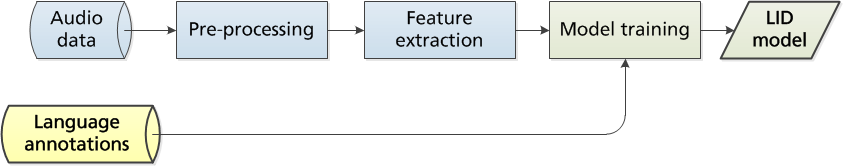
\includegraphics[width=1\textwidth]{images/process_training_lid.png}
		\caption{Schematic of the training procedure for language identification.}
		\label{fig:process_training_lid}
	\end{center}
\end{figure}
\begin{figure}
	\begin{center}
		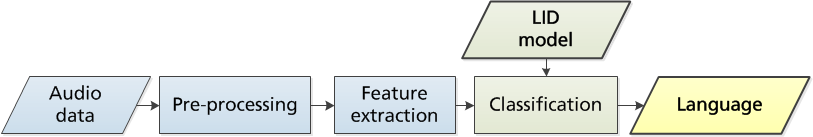
\includegraphics[width=1\textwidth]{images/process_classification_lid.png}
		\caption{Schematic of the classification procedure for language identification.}
		\label{fig:process_classification_lid}
	\end{center}
\end{figure}

Language identification has been extensively researched in the field of Automatic Speech Recognition since the 1980's. A number of successful algorithms has been developed over the years. An overview over the fundamental techniques is given by Zissman in \cite{zissman}.\\

Fundamentally, four properties of languages can be used to discriminate between them:
\begin{description}
	\item[Phonetics] The unique sounds that are used in a given language.
	\item[Phonotactics] The probabilities of certain phonemes and phoneme sequences.
	\item[Prosody] The ``melody'' of the spoken language.
	\item[Vocabulary] The possible words made up by the phonemes and the probabilities of certain combinations of words.
\end{description}
Even modern systems mostly focus on phonetics and phonotactics as the distinguishing factors between languages. Vocabulary is sometimes exploited in the shape of language models.\\

In ASR, the standard technique for language identification is Parallel Phone Recognition followed by Language Modeling (PPRLM). In this approach, acoustic and language models are trained for each language (or, in some cases, only the language models are different and just one acoustic model is used) . Unseen examples are then run through each model or combinations thereof, and the result with the highest likelihood determines the language (e.g. \cite{lid_li_ma} and \cite{lid_matejka}).\\

Other approaches directly train models for each language on the feature vectors (e.g. GMMs). This technique can be considered a ``bag of frames'' approach, i.e. the single data frames are considered to be statistically independent of each other. The trained models then describe probability densities for certain acoustic characteristics of each language. GMM approaches used to perform worse than their PPRLM counterparts, but the development of new features has made the difference negligible \cite{singer}. They are, in general, easier to implement since only audio examples and their language annotations are required. Allen et al. \cite{allen} report results of up to $76.4\%$ accuracy for ten languages. Different backend classifiers, such as Multi-Layer Perceptrons (MLPs) and Support Vector Machines (SVMs) \cite{campbell}, have also been used successfully instead of GMMs.\\

%HERE??
In this work, an approach that trains directly on the acoustic characteristics using i-vector extraction and SVMs is presented. The modifications to the general processing chain are presented in figures \ref{fig:process_training_lid} and \ref{fig:process_classification_lid}.
Additionally, a second approach based on phoneme posteriorgrams is tested. Statistics from the posteriorgrams are calculated, and then a second model is trained on these. Similar methods have been developed in ASR: Berkling presented an approach that uses sequences of recognized phonemes to discriminate between two languages (English and German), either with statistical modeling or with Neural Networks \cite{phdthesis:berkling_phd}. Mean errors of $0.12$ and $0.07$ on unseen data are achieved for the statistical approach and the Neural Network approach respectively when enough training data is available.\\

Li, Ma, and Lee present a system where acoustic inputs are tokenized into acoustic words, which do not necessarily correspond to phonetic n-grams. Then, language classifiers are trained on statistics of the acoustic words \cite{lid_li_ma_lee}. They obtain an equal error rate of $0.05$ for six languages using a universal phoneme recognizer for tokenization and SVMs for backend language recognition. Peche et al. \cite{peche} attempt a similar approach on languages with limited resources. The performance remains good even when only acoustic models trained on different languages are used.
In all of these approaches, tokenization of some sort is performed using the acoustic models. Since phoneme recognition on singing is still relatively unreliable, statistics are calculated directly on the phoneme posteriors in this work.\\

For evaluation, all test examples are classified into exactly one language class. Then, the accuracy (i.e. the average retrieval) is calculated:
 \begin{equation}
    Accuracy = \frac{TP}{N}
 \end{equation}  
 where $TP$ are the True Positives, and $N$ is the number of all documents. In ASR, the average cost measure as recommended in \cite{nist_cavg} is also used widely now; however, to remain in line with other sung language identification approaches such as those described in chapter \ref{chap:sota}, the accuracy was still used in this work.\\
 
 In both approaches, the \textit{NIST2003LRE} and \textit{OGIMultilang} corpora were used for testing the algorithms on speech, and the \textit{YTAcap} data set was used for singing (see chapter \ref{chap:datasets}). All results are obtained using 5-fold cross-validation - i.e., models are trained on 4/5 of each data set, then the remaining 1/5 is classified with the model. This is done 5 times until each utterance has been classified. This was necessary because the data sets are relatively small, and separating them into training and test sets would not have provided enough results for a meaningful evaluation.




\section{Sung language identification using i-vectors}
%known speakers - unknown speakers - whole documents


As described in section \ref{subsec:tech_ivector}, i-vector extraction is a feature dimension reduction technique that was originally developed for speaker recognition, but has since then been employed successfully for other tasks, including language identification. After the publication of this approach for i-vector extraction for sung language identification, it also started being used for other MIR tasks, such as artist recognition and similarity calculation \cite{eghbal-zadeh1}\cite{eghbal-zadeh2}.

\subsection{Proposed system}
\label{sec:system}
Figure \ref{fig:lid_ivectors} shows a rough overview over the i-vector classification system. 
%\begin{figure}[ht]
%\centerline{\includegraphics[scale=0.3]%{overview.png}}
%\caption{\label{fig:overview}{\it Overview of the steps of our classification system.}}
%\end{figure}
\begin{figure*}
	\begin{center}
		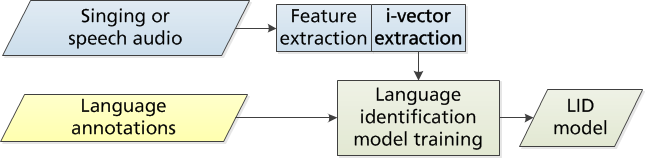
\includegraphics[width=.7\textwidth]{images/lid_ivectors.png}
		\caption{Overview of the process for language identification using i-vector extraction.}
		\label{fig:lid_ivectors}
	\end{center}
\end{figure*}

A number of features were extracted from each audio file. Table \ref{tab:ivec_configs} shows an overview over the various configurations used in training.
\begin{table}[h!tbp]
\scriptsize
  \begin{center}
     \begin{tabular}{|c|c|c|}\hline
     Name & Description & Dimensions \\ \hline
      MFCC  & MFCC, 20 coefficients & 20 \\
      MFCCDELTA  & MFCC, 20 coefficients, deltas and double-deltas & 60 \\
      MFCCDELTASDC  & MFCCDELTA+SDC & 117 \\
      SDC  & SDC with configuration $7-1-3-7$ & 91 \\
      RASTA-PLP & PLP with RASTA processing, model order 13 with deltas and double-deltas & 39 \\
      RASTA-PLP36  & PLP with RASTA processing, model order 36 with deltas and double-deltas  & 96 \\
      PLP  & PLP without RASTA processing, model order 13 deltas and double-deltas  & 39 \\
      COMB & PLP+MFCCDELTA & 99 \\ \hline
    \end{tabular}
  \end{center}
    \caption{{Feature configurations used in language identification training.}}
  \label{tab:ivec_configs}
\end{table}

%For classification, Multi-Layer Perceptrons (MLPs) and Support Vector Machines (SVMs) are tested. The MLPs are fixed at three layers, with the middle layer having a dimension of 256. Additional layers do not improve the result. A larger middle layer only improves it slightly. 
For classification, Support Vector Machines (SVMs) are tested. The SVM parameters are determined using a grid-search. For each of the data sets, all feature combinations listed in table \ref{tab:ivec_configs} are tested directly and with i-vector processing.\\


\subsection{Experiments with known speakers}
In the first experiment, SVM models are trained on randomly selected folds of the training data sets. This means that recordings by the same speaker are spread out between the training and test data sets. In theory, i-vectors could be particularly susceptible to capturing speaker characteristics instead of language characteristics, leading to evaluation results that are not representative of results for unknown speakers. However, this effect is often ignored in literature \cite{Martin2010}. There are use cases where taking speaker characteristics into account can actually contribute to the language identification accuracy - i.e., when detection is performed on data where some of the speakers are known in advance.

%\begin{figure}[h]
%       \centering
%      \begin{subfigure}[c]{0.3\textwidth}
%                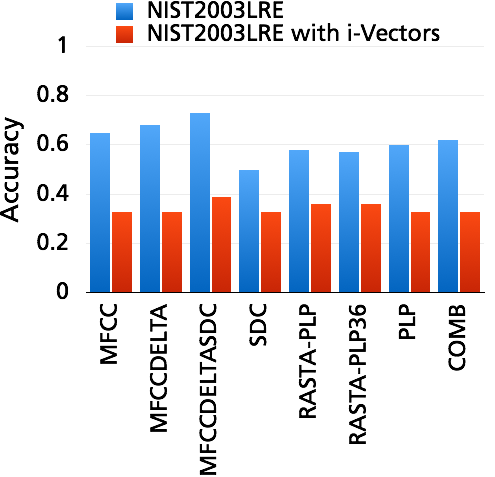
\includegraphics[width=\textwidth]{images/lid_exp1_nist.png}
%                \caption{NIST2003LRE}
%                \label{fig:lid_exp1_nist}
%        \end{subfigure}%
%        \begin{subfigure}[c]{0.3\textwidth}
%                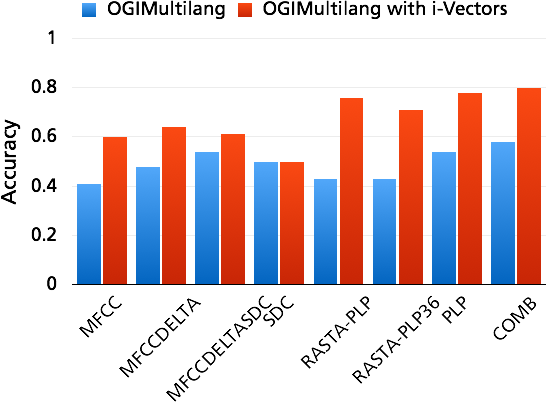
\includegraphics[width=\textwidth]{images/lid_exp1_ogi.png}
%                \caption{OGIMultilang}
%                \label{fig:exp1_ogi}
%        \end{subfigure}
%                \begin{subfigure}[c]{0.3\textwidth}
%                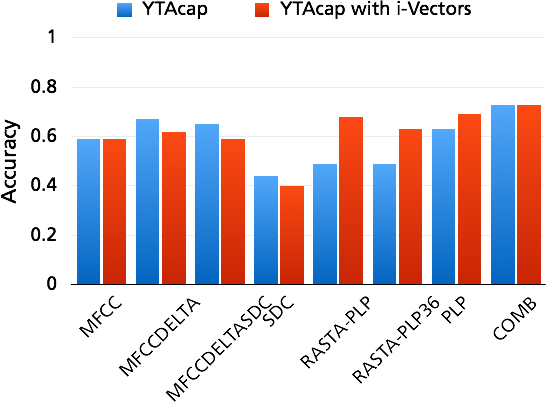
\includegraphics[width=\textwidth]{images/lid_exp1_yt.png}
%                \caption{YTAcap}
%                \label{fig:exp1_yt}
%        \end{subfigure}
%        \caption{Results using MLP models on all three language identification data sets, with or without i-vector processing.}\label{fig:lid_exp1}
%\end{figure}
%
%The results for the MLP training on the \textit{NIST2003LRE}, \textit{OGIMultilang}, and \textit{YTAcap} data sets are shown in figure \ref{fig:lid_exp1} in terms of accuracy (average retrieval when all documents are classified into exactly one language). \\
%As shown in figure \ref{fig:lid_exp1_nist}, the MLP does not produce good results on the \textit{NIST2003LRE} database for any of the feature combinations. \textit{NIST2003LRE} is the smallest of the data sets by a large margin. Since a relatively high-dimensional model is used, this is probably a case of overtraining. The i-vector processing step reduces the training data even further, thus aggravating the problem.\\
%The \textit{OGIMultilang} data set contains roughly 4 times as much data as the \textit{NIST2003LRE} set. With enough data, training an MLP classifier works a lot better. Without i-vector processing, this approach still only reaches about 52\% accuracy. i-Vector extraction improves the system massively. The best feature configurations are RASTA-PLP (82\%), PLP (80\%), and COMB (80\%).\\
%As with all other experiments, the task becomes harder when attempted on singing data. The results on the \textit{YTAcap} data set are worse than those on \textit{OGIMultilang}, even though they contain a similar amount of data. The best result without i-vector extraction is still obtained using the COMB feature configuration at 56\% accuracy. Similar to the \textit{OGIMultilang} experiment, i-vector extraction yields a large improvement. COMB remains the best configuration, now at 77\% accuracy.\\

\begin{figure}[h]
       \centering
      \begin{subfigure}[c]{0.3\textwidth}
                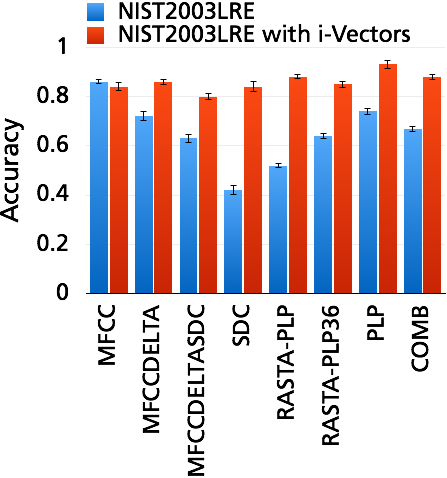
\includegraphics[width=\textwidth]{images/lid_exp1a_nist.png}
                \caption{NIST2003LRE}
                \label{fig:lid_exp1a_nist}
        \end{subfigure}%
        \begin{subfigure}[c]{0.3\textwidth}
                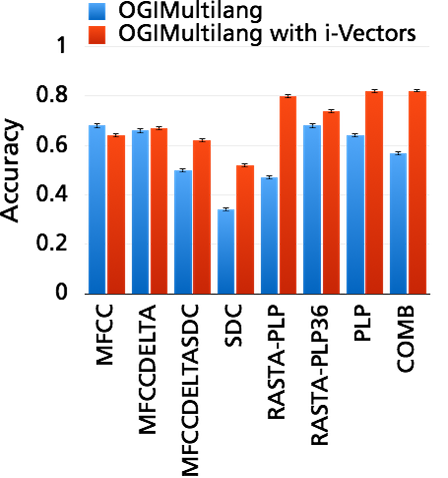
\includegraphics[width=\textwidth]{images/lid_exp1a_ogi.png}
                \caption{OGIMultilang}
                \label{fig:exp1a_ogi}
        \end{subfigure}
                \begin{subfigure}[c]{0.3\textwidth}
                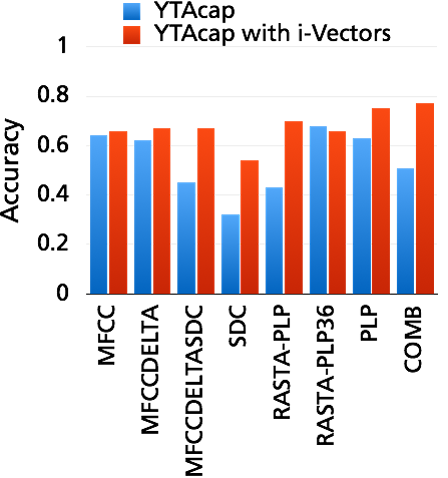
\includegraphics[width=\textwidth]{images/lid_exp1a_yt.png}
                \caption{YTAcap}
                \label{fig:exp1a_yt}
        \end{subfigure}
        \caption{Results using SVM models on all three language identification data sets, with or without i-vector processing, with speakers shared between training and test sets (error bars represent standard error over training folds).}\label{fig:lid_exp1a}
\end{figure}


Figure \ref{fig:lid_exp1a} shows the results for the SVM models trained on the \textit{NIST2003LRE}, \textit{OGIMultilang}, and \textit{YTAcap} data sets. In general, these models are able to capture the language boundaries well.\\

SVMs produce good results on the \textit{NIST2003LRE} data set for all of the features. They are able to discriminate very well on this small, clean data set. The best result with i-vector processing is $86\%$ accuracy for MFCC features. When using i-vectors, a 93\% accuracy is achieved with PLP features. This may, in fact, be close to the upper bound for the classification here; further analysis shows that misclassified recordings often mainly consist of laughter or very few words.\\

The \textit{OGIMultilang} corpus is roughly four times as big and more varied than the \textit{NIST2003LRE} corpus, making it harder to classify. As shown, the high-dimensional pure features do not perform as well as on \textit{NIST2003LRE}, with a maximum accuracy of 68\% for MFCCs and RASTA-PLPs with 36 coefficients. Using i-vector extraction improves the result by a large margin. Feature-wise, PLPs without RASTA processing work best at a result of 82\% accuracy. 
%CHECK!!!
MFCC and SDC features did not work quite as well, but did not hurt the result either when combined with PLPs (COMB result). It is interesting to see that the i-vector extraction decreased the results for MFCCs, the feature that worked best without it.\\

%CHECK!!
As with all other experiments, the task becomes harder when attempted on singing data. Similar to the \textit{OGIMultilang} corpus, the \textit{YTAcap} corpus provides very complex and varied data. The same effects occur with the direct feature training here, too: RASTA-PLPs with 36 coefficients provide the best results, but the accuracy is not very high at 68\%. i-Vector extraction once again serves to improve the result. The highest results when using i-vector extraction is a 75\% accuracy when using PLP without RASTA processing, or 77\% for the COMB configuration.
The same experiment was also conducted with MLP classifiers (see \cite{kruspe_lid2}), but they generally performed worse than their SVM counterparts. In the case of the small \textit{NIST2003LRE} data set, strong overfitting effects were observed.

\subsection{Experiments with unknown speakers}

In order to find out what influence the speaker characteristics had on the result, the same experiments were then repeated with training and evaluation sets that strictly separated speakers. This experiment was not performed for the \textit{NIST2003LRE}�corpus because no speaker information is available for it. Since the SVM models performed better in the previous experiment, only these models were tested.

\begin{figure}[h]
       \centering
        \begin{subfigure}[c]{0.4\textwidth}
                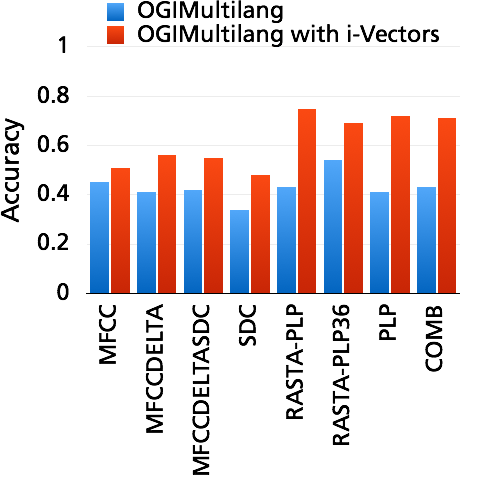
\includegraphics[width=\textwidth]{images/lid_exp2_ogi.png}
                \caption{OGIMultilang}
                \label{fig:exp2_ogi}
        \end{subfigure}
                \begin{subfigure}[c]{0.4\textwidth}
                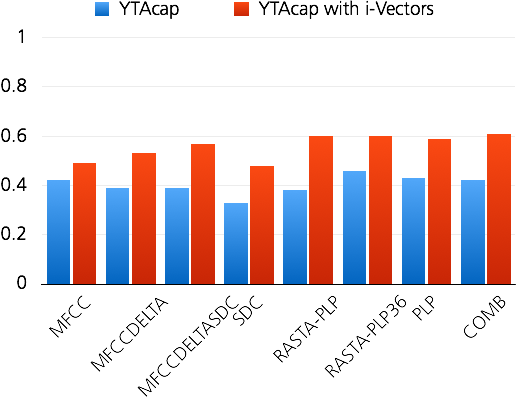
\includegraphics[width=\textwidth]{images/lid_exp2_yt.png}
                \caption{YTAcap}
                \label{fig:exp2_yt}
        \end{subfigure}
        \caption{Results using SVM models, with or without i-vector processing, with speakers separated between training and test sets (error bars represent standard error over training folds).}\label{fig:lid_exp2}
\end{figure}

The results are shown in figure \ref{fig:lid_exp2}. In general, all configurations perform worse, indicating that some of the characteristics learned by the models come from the speakers rather than the languages. Apart from this, the general trends for the features remain the same, and i-vector extraction still improves the over-all results.
On the \textit{OGIMultilang} corpus, the best result is still obtained with RASTA-PLP features and i-vector processing, but the accuracy falls by around 8 percent points to $75\%$. On \textit{YTAcap}, the effect is even worse: From an accuracy of $77\%$ with the mixed condition, the result decreases to $61\%$ for the separated condition. The reason for this is probably the wider signal variety in singing as opposed to speech; additionally, \textit{YTAcap} also possesses a wider range of recording conditions than the controlled telephone conditions of \textit{OGIMultilang}. Arguably, the solution for this effect would be the use of larger training data sets, which would be able to cover these acoustic and performance conditions better. Conversely, as the previous results show, the approach produces better results when an application scenario can be limited to a range of known speakers, or at least recording conditions (as in the \textit{NIST2003LRE} experiment).


%TODO: info about speakers and material per speaker
\subsection{Experiments with utterances combined by speakers}

All previous experiments were performed on relatively short utterances of a few seconds in duration. In many application scenarios, much more audio data is available to make a decision about the language. In particular, songs are usually a few minutes in length, and in many cases, only one result per document (= song) is required.
For this reason, results for the \textit{YTAcap} data set are taken from the previous experiment and a majority voting decision is made for each song (and therefore also for each singer). For the \textit{OGIMultilang} corpus, results for all utterances by the same speaker are aggregated in the same fashion, resulting in similar durations of audio. (Again, this experiment was not performed with the \textit{NIST2003LRE} corpus due to the lack of speaker information).\\

\begin{figure}[h]
       \centering
           \begin{subfigure}[c]{0.4\textwidth}
                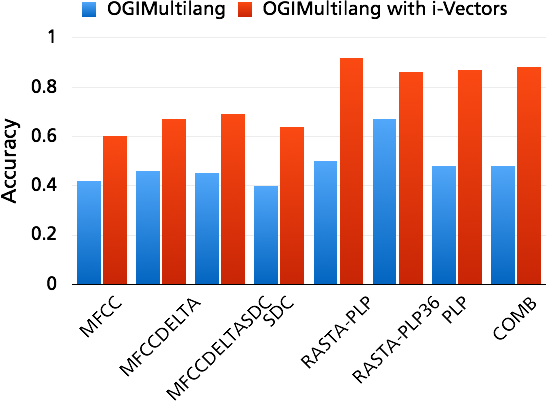
\includegraphics[width=\textwidth]{images/lid_exp3_ogi.png}
                \caption{OGIMultilang}
                \label{fig:exp3_ogi}
        \end{subfigure}
                \begin{subfigure}[c]{0.4\textwidth}
                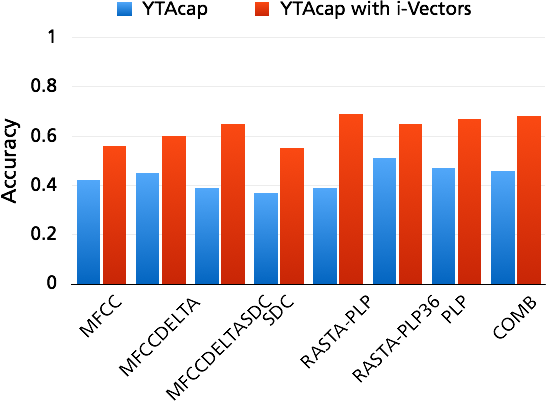
\includegraphics[width=\textwidth]{images/lid_exp3_yt.png}
                \caption{YTAcap}
                \label{fig:exp3_yt}
        \end{subfigure}
        \caption{Document-wise results using SVM models, with or without i-vector processing (error bars represent standard error over training folds).}\label{fig:lid_exp3}
\end{figure}

The results are shown in figure \ref{fig:lid_exp3}. Overall, aggregation of multiple utterances by the same speakers balances out some of the speaker-specific effects seen in the previous experiment. Taking more acoustic information into account, the models are able to determine the language with higher accuracy.
On the \textit{OGIMultilang} corpus, the result is even better than on the condition with known speakers. The best result rises from $75\%$ accuracy for short utterances to $92\%$ for the aggregated documents (both with the RASTA-PLP feature). On the \textit{YTAcap} data sets, the aggregated result is $69\%$ (compared to $60\%$ for line segments).
As suggested in the previous section, the approach produces results that are usable in practice when the problem can be narrowed down, e.g. to known speakers or recording conditions. As this experiment shows, useful results can also be obtained when longer sequences are available for analysis. 




%nicht n�tig f�r nist - kleine datenmengen gehen so mit svm. bei mlp aber overfitting.
%ogi: ivec erh�ht Ergebnis massiv. besser als irmfsp (warum?)
%yt: �hnlich ogi. Ergebnisse > sota. 
%features: plp gut, am besten ohne Rasta (warum?). mehr coeffs bringen aber nichts. mfcc f�r sich auch gut, mit delta noch besser, teilweise auch mit sdc.
%combi aus plp_norasta und mfccdelta funktioniert am besten - 2 verschiedene Aspekte abgedeckt (warum?)
%insgesamt: schnelleres training und weniger Speicherplatz als volle features, Irrelevanz reduziert. �hnliche Ergebnisse wie pprlm, aber viel einfacher. weniger Annotationen und leichter zu implementieren.




\section{Sung language identification using phoneme recognition posteriors}\label{sec:lid_stats}
Another developed approach is based upon phoneme statistics derived from phoneme posteriorgrams. To obtain representative statistics for model training, relatively long observations are necessary, but, as described in the previous section, this is the case for many applications, for example when considering song material (e.g. songs of 3-4 minutes in duration). On the other hand, phoneme posteriorgrams need to be calculated for a number of other tasks, such as keyword spotting or lyrics-to-audio alignment. \\

\begin{figure*}
	\begin{center}
		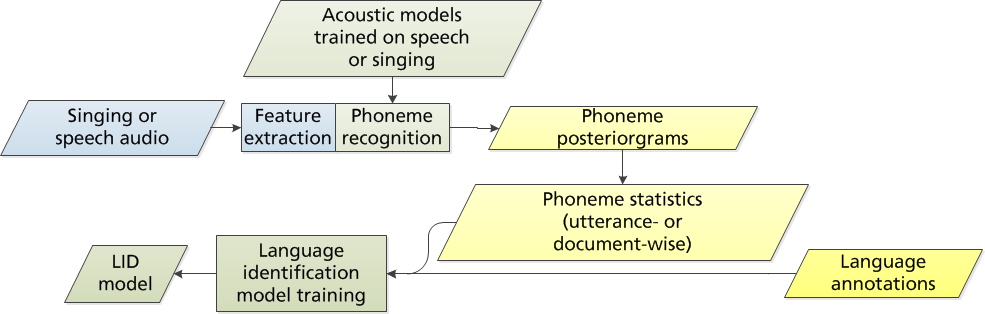
\includegraphics[width=1\textwidth]{images/process_lid_stats.png}
		\caption{Overview of the process for language identification using phoneme statistics.}
		\label{fig:lid_statistics_process}
	\end{center}
\end{figure*}

An overview of the approach is shown in figure \ref{fig:lid_statistics_process}. Posteriorgrams are generated on the test data sets \textit{YTAcap} and \textit{OGIMultilang} using the acoustic models trained on the \textit{TIMIT} speech data set and on the \textit{DAMP} singing data set as described in section \ref{sec:phonerec_acap}. To facilitate the following language identification, phoneme statistics are then calculated in two different ways:
\begin{description}
  \item[Document-wise statistics]{Mean and variances of the phoneme likelihoods over whole songs or sets of utterances of a single speaker are calculated. This results in just two feature vectors per document (one for the means, one for the variances).}
  \item[Utterance-wise statistics]{Means and variances of the phoneme likelihoods over each utterance are calculated (or, in the case of \textit{YTAcap}, over each song segment). For further training, the resulting vectors for each speaker/song (= document) are used as a combined feature matrix. As a result, no overlap of speakers/songs is possible between the training and test sets.}
\end{description}
Naturally, relatively long recordings are necessary to produce salient statistics. For this reason, the aggregation by speaker/song is done in both cases rather than treating each utterance separately.
Then, Support Vector Machine (SVM) models are trained on the calculated statistics in both variants with the three languages as annotations. Unknown song/speaker documents can then be subjected to the whole process and classified by language.\\
%Again, all results are obtained using 5-fold cross-validation - i.e., SVMs are trained on 4/5 of each corpus, then the remaining 1/5 is classified with the model. This is done 5 times until each song/speaker document has been classified.

\subsection{Language identification using document-wise phoneme statistics}
In the first experiment, SVM classifiers are trained on the document-wise phoneme statistics, and classification is also performed on a document-wise basis (i.e., only one mean and one variance vector per document). The results are shown in figure \ref{fig:lid_statistics_res1}.
On the singing test set, results are worst when using acoustic models trained on \textit{TIMIT} at just $53\%$ accuracy, and become better when using the model trained on the ``songified'' \textit{TIMIT} variant \textit{TimitM} (see section \ref{sec:phonerec_songify}), or on the small selection of the singing training set \textit{DampBB\_small} at an accuracy of $59\%$ each. The best result of $63\%$ accuracy is achieved when the models are trained on the full singing data set.
Surprisingly, the results on the \textit{OGIMultilang} corpus also improve from $75\%$ with the \textit{TIMIT} models to $84\%$ using the \textit{DampB} models. Since \textit{TIMIT} is a very ``clean'' data set, training on the singing corpus provides some more phonetic variety, acting as a sort of data augmentation. This is especially important in this context where phonemes are recognized in three different languages.
On both corpora, there is no noticeable bias of the confusion matrix - i.e., the confusions are spread out evenly. This is particularly interesting when considering that the acoustic models were trained on English speech or singing only.
%\begin{figure}[h]
 %       \centering
  %      \begin{subfigure}[c]{0.25\textwidth}
  %              \includegraphics[width=\textwidth]%{figs/stat_acc.png}
   %             \caption{Accuracy}
   %             \label{fig:stat_acc}
  %      \end{subfigure}%
   %     ~ %add desired spacing between images, e. g. ~, \quad, \qquad, \hfill etc.
          %(or a blank line to force the subfigure onto a new line)
   %     \begin{subfigure}[c]{0.25\textwidth}
     %           \includegraphics[width=\textwidth]%{figs/stat_cavg.png}
   %             \caption{Average cost}
  %              \label{fig:stat_cavg}
 %       \end{subfigure}
 %       \caption{Results using document-wise phoneme statistics generated with various acoustic models.}\label{fig:res_stat}
%\end{figure}

\begin{figure*}
	\begin{center}
		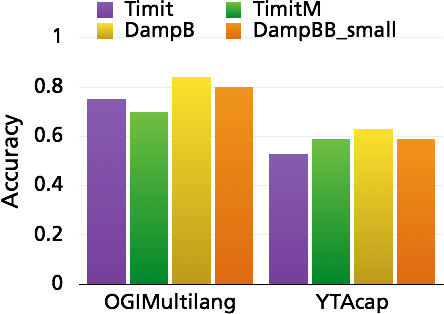
\includegraphics[width=.4\textwidth]{images/lid_statistics_res1.png}
		\caption{Results using document-wise phoneme statistics generated with various acoustic models (error bars represent standard error over training folds).}
		\label{fig:lid_statistics_res1}
	\end{center}
\end{figure*}

\subsection{Language identification using utterance-wise phoneme statistics}
Next, language identification was performed with models trained on the statistics of each utterance contained in the document. The recognition process is still performed on the whole document. The results are reported in figure \ref{fig:lid_statistics_res2}.
Phoneme statistics are not as representative when computed on shorter inputs, but they provide more information for the backend model training when utilized as a combined feature matrix for a longer document. The results on singing improve slightly (significant with $p<0.1$) to $63\%$ accuracy with the acoustic model trained on the small singing corpus (\textit{DampBB\_small}) and decrease insignificantly for the \textit{DampB} model ($61\%$). However, on the speech corpus, the best result rises to $90\%$.
%why??
%\setlength{\belowcaptionskip}{-0.3cm}
%\begin{figure}[h]
 %       \centering
 %       \begin{subfigure}[c]{0.25\textwidth}
  %              \includegraphics[width=\textwidth]%{figs/stats_acc.png}
  %              \caption{Accuracy}
 %               \label{fig:stats_acc}
%        \end{subfigure}%
 %       ~ %add desired spacing between images, e. g. ~, \quad, \qquad, \hfill etc.
          %(or a blank line to force the subfigure onto a new line)
 %       \begin{subfigure}[c]{0.25\textwidth}
 %               \includegraphics[width=\textwidth]%{figs/stats_cavg.png}
 %               \caption{Average cost}
  %              \label{fig:stats_cavg}
  %      \end{subfigure}
  %      \caption{Results using utterance-wise phoneme statistics generated with various acoustic models.}\label{fig:res_stats}
%\end{figure}
%\setlength{\belowcaptionskip}{-0.1cm}
\begin{figure*}
	\begin{center}
		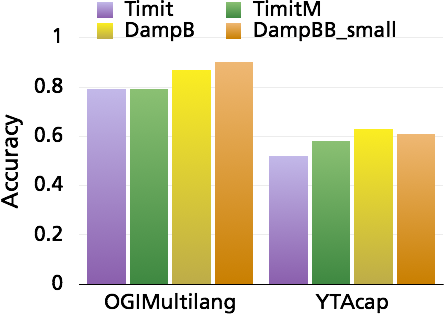
\includegraphics[width=.4\textwidth]{images/lid_statistics_res2.png}
		\caption{Results using utterance-wise phoneme statistics generated with various acoustic models.}
		\label{fig:lid_statistics_res2}
	\end{center}
\end{figure*}

\subsection{For comparison: Results for the i-vector approach}
For comparison, models from the previous approach were also trained on the same time scales. i-Vectors were calculated on the utterance- or the document-wise scale. This was done for PLP and MFCC features. The resulting i-vectors were then used to train SVMs in the same manner as in the previous experiments. (The difference here is that the models are already trained on the aggregated i-vectors, either with those for a whole document or with all i-vectors of the utterances constituting each document aggregated). The results are shown in figure \ref{fig:lid_statistics_res3}.\\

The best result obtained on \textit{YTAcap} data set is $68\%$ accuracy. This is only 5 percent points higher than the approach based on phoneme statistics, which is easier to implement. On the \textit{OGIMultilang} corpus, the difference is only 3 percent points ($93\%$). Of course, the advantage of the i-vector approach is that it can also be performed on much shorter inputs.\\

\begin{figure*}
	\begin{center}
		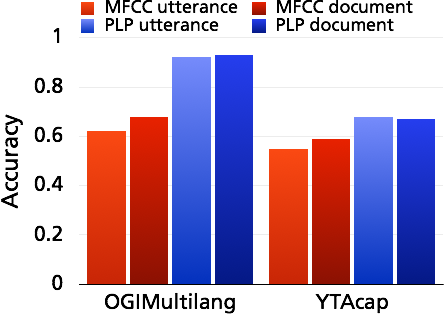
\includegraphics[width=.4\textwidth]{images/lid_statistics_res3.png}
		\caption{Results using utterance- and document-wise i-vectors calculated on PLP and MFCC features (error bars represent standard error over training folds).}
		\label{fig:lid_statistics_res3}
	\end{center}
\end{figure*}
%\begin{figure}[h]
 %       \centering
%        \begin{subfigure}[c]{0.25\textwidth}
 %               \includegraphics[width=\textwidth]%{figs/ivec_acc.png}
  %              \caption{Accuracy}
   %             \label{fig:ivec_acc}
  %      \end{subfigure}%
  %      ~ %add desired spacing between images, e. g. ~, \quad, \qquad, \hfill etc.
          %(or a blank line to force the subfigure onto a new line)
 %       \begin{subfigure}[c]{0.25\textwidth}
 %               \includegraphics[width=\textwidth]%{figs/ivec_cavg.png}
 %               \caption{Average cost}
  %              \label{fig:ivec_cavg}
  %      \end{subfigure}
  %      \caption{Results using utterance- and document-wise i-vectors calculated on PLP and MFCC features.}\label{fig:res_ivec}
%\end{figure}

\section{Conclusion}\label{sec:lid_conclusion}
In this section, two approaches to singing language identification were presented: One based on i-vector processing of audio features, and one based on the computation of phoneme statistics from posteriorgrams. In both cases, machine learning models were trained on the resulting data.\\

In the first approach, PLP, MFCC, and SDC features are extracted from audio data, and then run through an i-vector extractor. The generated i-vectors are then used as inputs for SVM training. The basic idea behind the i-vector approach is the removal of language-independent components of the signal. This effectively reduces irrelevance to the language identification tasks and also reduces the amount of training data massively.
The smallest data set is the \textit{NIST2003LRE} corpus.
%No feature configuration achieves good results when using the MLP backend. In this case, the small size of the corpus leads to overtraining. i-Vector processing only amplifies this problem by reducing the amount of data even further.
The SVM backend produces good results of up to 93\% for PLP features with i-vector extraction.\\

The \textit{OGIMultilang} corpus is a much bigger speech corpus. Training without i-vector extraction does not work well for any feature configuration. The best accuracy for this scenario was 68\%. Results of up to 83\% are achieved with i-vector processing. 
%There is no large difference between SVM and MLP training, with SVMs having just a slight advantage.\\
Language identification for singing was expected to be a harder task than for speech due to the factors described in section \ref{sec:sota_speechtosinging}. The results on the \textit{YTAcap} corpus turn out to be somewhat worse than those for the \textit{OGIMultilang} corpus, which is of similar size. Once again, i-vector extraction improves the results from 63\% to 73\%.\\

The same experiment is repeated with no speaker overlap between training and test sets. The results fall significantly ($p<0.0001$), indicating speaker influence on the model training. In a third experiment, the results are aggregated into documents by each speaker, which again leads to improved results. The best accuracy on \textit{OGIMultilang} is $92\%$, while on \textit{YTAcap}, it is $69\%$. Both experiments demonstrate that useful results can be obtained when limiting the task, e.g. by training on a set of known speakers or recording conditions, or by analyzing documents of longer durations. Alternatively, a wider range of speakers in the training data would lead to models that generalize better.\\

Overall, i-vector extraction reduces irrelevance in the training data and thereby leads to a more effective training. As additional benefits, the training process itself is much faster and less memory is used due to its data reduction properties. Most of the state-of-the-art approaches are based on PPRLM, which requires phoneme-wise annotations and a highly complex recognition system, using both acoustic and language models. In this respect, this system is easier to implement and merely requires language annotations.\\

The second presented method is a completely new language identification approach for singing. It is based on the output of various acoustic models, from which statistics are generated and SVM models are trained. In contrast to similar approaches for speech, no voice tokenization is performed. Since phoneme recognition on singing is not always reliable, the statistics are calculated directly on the phoneme posteriorgrams, although this does not take any temporal information into account. The acoustic models are trained only on English-language material (speech and singing); it would be interesting to test this with multi-language training data. Due to the statistics-based nature of the approach, it is not suited for language identification of very short audio recordings.\\

The accuracy of the result for singing is somewhat worse than the results obtained with the i-vector based approach. However, this new approach is much easier to implement and the feature vectors are shorter. For many applications, such posteriors need to be extracted anyway and can efficiently be used for language identification when long observations are available. The best accuracy of $63\%$ is obtained with acoustic models trained on the \textit{DampB} singing corpus.\\

Interestingly, the best result on the \textit{OGIMultilang} speech corpus is also obtained with these acoustic models (and is only 3 percent points below the one obtained with the i-vector approach). This possibly happens because the singing corpora provide a wider range of phoneme articulations. It would be interesting to try out these acoustic models for other phoneme recognition tasks on speech where robustness to varied pronunciations is a concern.



